\chapter{Excitability Types: Integrators and Resonators}
\label{ch:excitability}

\textit{Excitability type is determined by the bifurcation that creates repetitive firing. SNIC onset yields Type~I neurons that can fire arbitrarily slowly, whereas Hopf onset yields Type~II neurons with a finite onset frequency and an intrinsic timescale.}

% ============================================================
\section{Two Roads to Repetitive Firing}
\label{sec:two-roads}
% ============================================================

As injected current increases, a neuron eventually leaves rest and enters repetitive firing. The key question is not merely \emph{whether} a limit cycle appears, but \emph{how} it appears, because the onset geometry already determines latency, threshold structure, and coding strategy.

The two dominant onset mechanisms are the \emph{saddle-node on an invariant circle}\index{saddle-node on invariant circle} (SNIC) and the \emph{Hopf bifurcation}\index{Hopf bifurcation}. \Cref{fig:excitability-types} summarizes the central qualitative difference.

\begin{figure}[h]
\centering
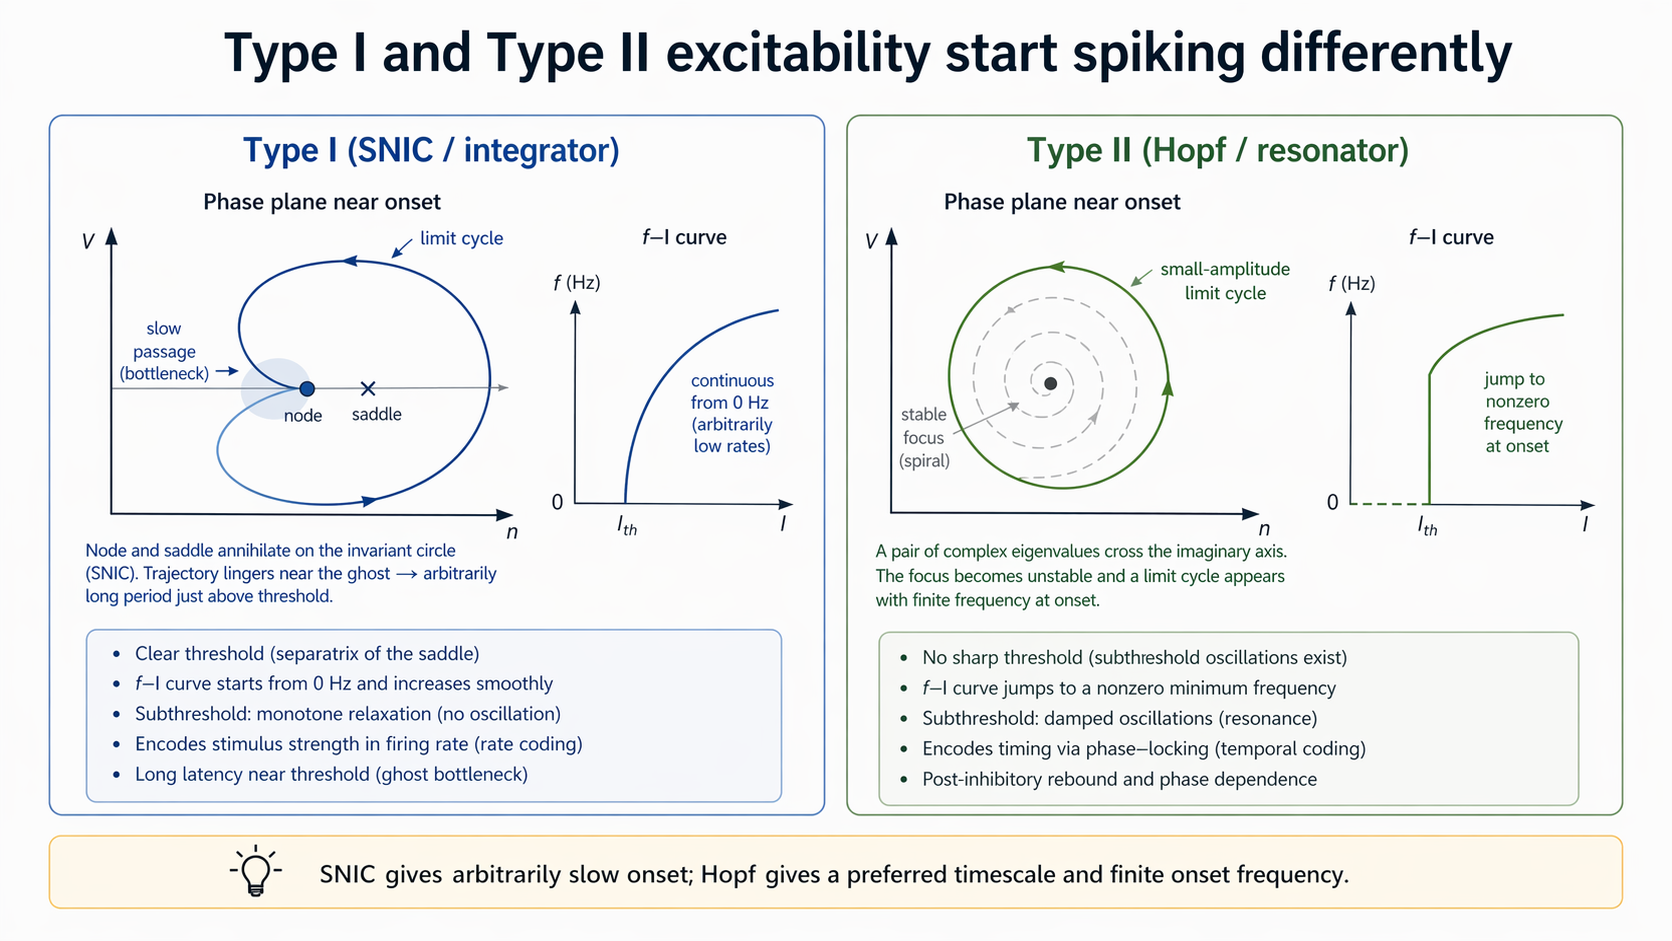
\includegraphics[width=\textwidth]{figures/mns-excitability-types.png}
\caption{Type~I and Type~II onset are distinguished by bifurcation geometry. SNIC onset creates arbitrarily slow firing through a bottleneck, whereas Hopf onset creates oscillation at a finite intrinsic frequency.}
\label{fig:excitability-types}
\end{figure}

% ============================================================
\section{Type I: Saddle-Node on Invariant Circle}
\label{sec:type-1}
% ============================================================

In a SNIC bifurcation, the resting state (a stable node) and a nearby saddle point sit on a closed curve in the phase plane. As the current increases, the node and saddle approach each other, collide, and annihilate---exactly as in the one-dimensional saddle-node (\cref{sec:saddle-node-1d}), except that now the annihilation happens on a circle. Once both fixed points are gone, trajectories travel around the entire circle: a limit cycle is born.

The distinctive feature of the SNIC is that the limit cycle's period is \emph{infinite} at onset. Just above the bifurcation, trajectories still pass slowly through the ghost of the annihilated fixed points, spending a long time in the bottleneck region. The resulting firing rate can be made arbitrarily small by bringing the current just above threshold. This gives a continuous, smooth $f$--$I$ curve that starts from zero.

\subsection{Properties of Type~I neurons}

Type~I neurons\index{Type I excitability} behave as \emph{integrators}\index{integrator}: they accumulate input over time and fire when enough has been collected. Their key properties are:

The $f$--$I$ curve is continuous at onset---the firing rate starts from zero and increases smoothly with current. There is a well-defined threshold, corresponding to the separatrix (the saddle's stable manifold) that exists just below the bifurcation. Subthreshold responses are mostly monotone rather than oscillatory: excitation pushes the state toward threshold and inhibition pulls it back. The neuron encodes stimulus intensity through its firing \emph{rate}: stronger input produces higher rates, with no preferred frequency.

Near threshold, the ghost of the saddle-node produces a long latency to the first spike---the neuron sits near rest for hundreds of milliseconds before firing. This latency decreases sharply as the current is increased.

% ============================================================
\section{Type II: Hopf Bifurcation}
\label{sec:type-2}
% ============================================================

In a Hopf bifurcation, the resting state (a stable spiral) loses stability as a pair of complex conjugate eigenvalues crosses the imaginary axis. The real part of the eigenvalues changes sign from negative to positive, and the stable spiral becomes an unstable spiral. Simultaneously, a limit cycle appears around the newly unstable fixed point.

In a \emph{supercritical} Hopf bifurcation, the limit cycle is stable and has small amplitude at birth, growing as the parameter moves further past the bifurcation. In a \emph{subcritical} Hopf, the limit cycle is unstable (it acts as a separatrix), and the neuron jumps abruptly to a large-amplitude oscillation. Either way, the limit cycle has a \emph{nonzero frequency} at onset, set by the imaginary part of the eigenvalues at the bifurcation.

\subsection{Properties of Type~II neurons}

Type~II neurons\index{Type II excitability} behave as \emph{resonators}\index{resonator}: they have a preferred frequency and respond best to inputs at that frequency. Their key properties are:

The $f$--$I$ curve has a discontinuity at onset---the firing rate jumps from zero to a minimum nonzero value. There is no clean threshold; subthreshold oscillations exist below the bifurcation (the stable spiral produces damped oscillations that can be excited by brief inputs). Inputs at the neuron's resonant frequency are preferentially amplified, while inputs at other frequencies are suppressed. The neuron encodes stimulus timing through phase-locking to periodic inputs.

Post-inhibitory rebound\index{post-inhibitory rebound} is a hallmark of resonators: a brief hyperpolarizing pulse can trigger a spike after the pulse ends, because the release from inhibition interacts with the subthreshold oscillation to push the voltage above threshold.

Close to Hopf onset, responses can be \emph{graded} rather than all-or-none: different perturbation amplitudes can produce different spike amplitudes or spike failures before the trajectory settles onto the limit cycle. Pulse timing also matters strongly: inputs that align with the intrinsic oscillation phase can trigger spikes efficiently, while off-phase pulses may be ineffective.

% ============================================================
\section{Global Orbit Geometry Near Threshold}
\label{sec:global-geometry}
% ============================================================

Local eigenvalue analysis explains stability, but global phase-plane structures determine threshold geometry and spike initiation pathways. Two important objects are heteroclinic and homoclinic orbits.

A \emph{heteroclinic orbit}\index{heteroclinic orbit} connects two different equilibria (typically along stable/unstable manifolds). A \emph{homoclinic orbit}\index{homoclinic orbit} leaves and returns to the same saddle equilibrium. In excitability models, these orbits organize transitions between rest, spike initiation, and large-amplitude oscillations.

Near SNIC regimes, the saddle's stable manifold forms the threshold manifold and its unstable manifold helps shape trajectories toward the spiking branch. Near Hopf regimes, threshold becomes less geometric and more phase dependent, because trajectories spiral and threshold cannot be summarized by a single voltage or a single separatrix curve.

Computationally, these global structures explain why two models with similar local linearization can still have very different spike-triggering behavior.

% ============================================================
\section{Reading Bifurcation Diagrams}
\label{sec:bif-diagrams}
% ============================================================

A bifurcation diagram plots equilibria and periodic orbits as a control parameter (often $I_{\text{ext}}$) varies. Solid branches denote stable solutions; dashed branches denote unstable ones. For Type~I onset (SNIC), the oscillation frequency approaches zero at threshold. For Type~II onset (Hopf), oscillations emerge at nonzero frequency.

In practice, three visual checks are especially useful:
\begin{enumerate}
  \item Track where the resting fixed point loses stability.
  \item Check whether oscillation amplitude appears continuously (supercritical Hopf) or by jump (subcritical Hopf / global transition).
  \item Check whether onset frequency tends to $0$ (SNIC-like) or stays finite (Hopf-like).
\end{enumerate}

These diagnostics are what connect numerical continuation plots to experimentally measurable $f$--$I$ curves, latency, and resonance.

% ============================================================
\section{Integrator versus Resonator: A Comparison}
\label{sec:comparison}
% ============================================================

The distinction between integrators and resonators is not merely a classification exercise---it reflects fundamentally different computational strategies.

\begin{center}
\renewcommand{\arraystretch}{1.4}
\begin{tabularx}{\textwidth}{@{}l X X@{}}
  \toprule
  \textbf{Property} & \textbf{Integrator (Type~I)} & \textbf{Resonator (Type~II)} \\
  \midrule
  Bifurcation & SNIC & Hopf \\
  $f$--$I$ onset & Continuous from 0 Hz & Jump to nonzero frequency \\
  Threshold & Well-defined separatrix & No sharp boundary \\
  Subthreshold dynamics & Monotone decay & Damped oscillations \\
  Preferred frequency & None (broadband) & Yes (resonance) \\
  Coding strategy & Rate coding & Temporal / coincidence coding \\
  Post-inhibitory rebound & Absent & Present \\
  Latency near threshold & Long (ghost effect) & Short \\
  \bottomrule
\end{tabularx}
\end{center}

\noindent The standard Hodgkin--Huxley model, with its original squid axon parameters at $6.3\,^\circ\text{C}$, exhibits Type~II behavior: the onset of firing involves a Hopf-like bifurcation, and the $f$--$I$ curve jumps to a nonzero frequency. However, varying the channel densities or temperature can shift the model to Type~I behavior. Biology is not locked into one class---different neurons in the brain use different strategies depending on their computational role.

\subsection{Threshold manifold versus threshold voltage}

For integrators close to SNIC, threshold is well approximated by a manifold (the stable manifold of a saddle): crossing it predicts spike initiation robustly. For resonators close to Hopf, this manifold picture weakens; threshold depends strongly on state-space phase and input timing. This is why ``threshold voltage'' is often variable in resonator-like neurons.

Computationally, this distinction clarifies why some neurons are well described by scalar threshold models, while others require at least two-dimensional state tracking.

% ============================================================
\section{Reduced Models}
\label{sec:reduced-models}
% ============================================================

Full conductance-based models have many parameters and are hard to analyze. Reduced models capture the essential dynamics in two variables, making phase-plane analysis tractable.

\subsection{The Izhikevich model}

The Izhikevich model\index{Izhikevich model} uses a quadratic voltage equation with a linear recovery variable:
%
\begin{align}
  \Cm\dot{v} &= k(v - v_r)(v - v_t) - u + I \label{eq:izh-v} \\[4pt]
  \dot{u} &= a\bigl[b(v - v_r) - u\bigr] \label{eq:izh-u}
\end{align}
%
with reset: if $v \geq v_{\text{peak}}$, set $v \leftarrow c$ and $u \leftarrow u + d$. The parameters $a, b, c, d$ control the timescale of recovery, the subthreshold behavior, the reset voltage, and the post-spike adaptation. By tuning these four parameters, the model can reproduce both Type~I and Type~II excitability, bursting, adaptation, and many other firing patterns observed in real neurons.

The model bridges the gap between the biophysical detail of Hodgkin--Huxley and the simplicity of integrate-and-fire. The quadratic nonlinearity in $v$ captures the essential positive feedback of sodium activation without requiring explicit gating variables.

\subsection{The theta model}

The \emph{theta model}\index{theta model} places the dynamics on a circle:
%
\begin{equation}
  \dot{\theta} = (1 - \cos\theta) + (1 + \cos\theta)\,I
  \label{eq:theta}
\end{equation}
%
A ``spike'' corresponds to $\theta$ passing through $\pi$. The circle topology means there is no need for an artificial reset rule---the system wraps around naturally. The theta model is the canonical normal form for the SNIC bifurcation. Below threshold ($I < 0$), there are two fixed points on the circle; above threshold ($I > 0$), they annihilate and the phase $\theta$ increases monotonically, producing periodic spiking.

\subsection{The resonate-and-fire model}

A complementary canonical model for resonators is the \emph{resonate-and-fire} model\index{resonate-and-fire model}. In complex notation:
%
\begin{equation}
  \dot z = (\lambda + i\omega_0)z + I(t),
  \label{eq:resonate-fire}
\end{equation}
%
with a spike emitted when $\\Re(z)$ crosses threshold, followed by reset. The parameter $\\omega_0$ sets intrinsic subthreshold oscillation frequency, and $\\lambda<0$ sets damping.

Unlike LIF-like integrators, this model explicitly captures phase-sensitive excitability, rebound, and frequency-selective response. It is therefore a convenient reduced model for Type~II-like dynamics when full conductance models are too costly.


\begin{chaptersummary}

\begin{center}
\renewcommand{\arraystretch}{1.6}
\begin{tabularx}{\textwidth}{@{}l X X@{}}
  \toprule
  \textbf{Concept} & \textbf{Equation / Property} & \textbf{Key Insight} \\
  \midrule
  SNIC bifurcation &
  Node + saddle annihilate on circle &
  Type~I: continuous $f$--$I$, arbitrarily low rate \\
  %
  Hopf bifurcation &
  Complex $\lambda$ cross imaginary axis &
  Type~II: nonzero onset frequency, resonance \\
  %
  Integrator &
  Rate coding, clear threshold &
  Accumulates input; fires when enough \\
  %
  Resonator &
  Temporal coding, damped oscillations &
  Responds best at preferred frequency \\
  %
  Global orbits &
  Heteroclinic / homoclinic geometry &
  Organize threshold and trajectory structure \\
  %
  Bifurcation diagram &
  Stable/unstable branches vs $I$ &
  Links phase-plane theory to measurable $f$--$I$ \\
  %
  Izhikevich model &
  $\Cm\dot{v} = k(v - v_r)(v - v_t) - u + I$ &
  Four parameters reproduce many patterns \\
  %
  Theta model &
  $\dot\theta = (1 - \cos\theta) + (1 + \cos\theta)I$ &
  SNIC normal form; no reset needed \\
  %
  Resonate-and-fire &
  $\dot z = (\lambda + i\omega_0)z + I$ &
  Canonical phase-sensitive resonator model \\
  \bottomrule
\end{tabularx}
\end{center}

\end{chaptersummary}

\begin{conceptquestions}
  \item Why does the SNIC bifurcation produce a continuous $f$--$I$ curve starting from zero, while the Hopf bifurcation produces a jump to a nonzero frequency? Connect your answer to the dynamics near the bifurcation.

  \item In a SNIC bifurcation, the period of the limit cycle is infinite at onset. Where does the trajectory spend most of its time near the bifurcation, and why?

  \item Explain the difference between a supercritical and a subcritical Hopf bifurcation. Which one produces a smooth transition to small-amplitude oscillations? Which produces an abrupt jump to large-amplitude spiking?

  \item A resonator neuron shows post-inhibitory rebound: a brief hyperpolarizing pulse can trigger a spike. Why does this happen, and why is it absent in integrators?

  \item An integrator neuron uses rate coding: stimulus intensity is encoded in firing rate. A resonator uses temporal coding: stimulus timing is encoded in spike timing relative to the input. Explain why each coding strategy follows naturally from the underlying bifurcation.

  \item Two excitatory inputs arrive at an integrator neuron, one $5\;\text{ms}$ after the other. Compare the neuron's response to the case where both inputs arrive simultaneously. Now repeat the comparison for a resonator neuron. How does the integration window differ?

  \item The comparison table lists ``preferred frequency: none'' for integrators and ``preferred frequency: yes'' for resonators. What physical feature of the subthreshold dynamics gives rise to a preferred frequency? Where does this frequency come from in terms of the eigenvalues?

  \item The standard Hodgkin--Huxley model is Type~II, but varying channel densities can make it Type~I. What does this tell you about the relationship between channel biophysics and excitability type?

  \item The Izhikevich model uses a quadratic nonlinearity $k(v - v_r)(v - v_t)$ instead of explicit gating variables. What biophysical process does this term approximate, and why is a quadratic sufficient?

  \item The theta model $\dot{\theta} = (1 - \cos\theta) + (1 + \cos\theta)I$ lives on a circle. Why does the circle topology eliminate the need for an explicit reset rule? What are the fixed points when $I < 0$, and what happens to them when $I > 0$?

  \item What is the practical difference between saying ``threshold is a manifold'' and ``threshold is phase dependent''? Give one implication for experiments with brief pulses.

  \item In a bifurcation diagram, how would you distinguish a SNIC-like onset from a Hopf-like onset using frequency behavior near threshold?

  \item A neuron in the brain might switch between integrator and resonator behavior depending on neuromodulatory state. What biophysical change could produce this switch? Give an example involving a specific channel type.

  \item The LIF model from \cref{ch:lif} has a continuous $f$--$I$ curve starting from zero. Based on this, is the LIF model Type~I or Type~II? What bifurcation does the threshold-and-reset rule implicitly implement?
\end{conceptquestions}
